\documentclass{emulateapj}
\newcommand{\vdag}{(v)^\dagger}
\newcommand{\myemail}{tleung@astro.cornell.edu}
%\slugcomment{{\sc Accepted to ApJ:} August 1, 2006}
\usepackage{amsmath}
\usepackage{natbib}
\citestyle{aa}
\shorttitle{Study of a strongly lensed type-2 quasar host SMG at $z$ = 2.221}
%\shortauthors{Leung and Riechers}

\begin{document}
\title{CO($J$ = 3 $\rightarrow$ 2) observation in a strongly lensed type-2 quasar host SMG at $z$ = 2.221 with
continuum detection in the foreground lensing FR-II radio galaxy at $z$ = 0.685}
\author{No name}
%\author{T. K. Daisy Leung\altaffilmark{1} and Dominik R. Riechers\altaffilmark{2}}
%\affil{Astronomy Department, Cornell Unviersity}
%\altaffiltext{1}{tleung@astro.cornell.edu}
%\altaffiltext{2}{dr@astro.cornell.edu}

\begin{abstract}
We report the detection of CO($J$ = 3 $\rightarrow$ 2) line emission in SMM J0939+8315 ($z$ = 2.221), a
strongly lensed high-redshift submillimeter galaxy (SMG) hosting a type-2 quasar using
the Combined Array for Research in Millimeter-wave Astronomy (CARMA). This lensing system consists of a
foreground FR-II radio galaxy and a companion galaxy at $z$ = 0.685. We perform lens modeling on the Submillimeter Array (SMA) 1 mm dust continuum, resulting a
lensing magnification factor of $\mu=$9.7 $\pm$ 1.4. This allows us to place constraints on the intrinsic properties
of the cold gas and dust in the interstellar medium (ISM) of the background quasar host SMG. Prior to correcting for lensing amplification, we measure the
velocity-integrated CO($J$ = 3 $\rightarrow$ 2) line intensity of $I_{\rm CO(3-2)}$ = (14.6 $\pm$ 0.9) Jy km s$^{-1}$,
corresponding to a lensing-corrected CO($J$ = 1 $\rightarrow$ 0) line luminosity of $L^{\prime}_{\rm CO(1-0)}$ = (4.1 $\pm$ 0.9) $\times$ 10$^{10}$ K km s$^{-1}$ pc$^2$. This
translates to a molecular gas mass of $M_{\rm gas}$ = 3.3 $\times$ 10$^{10}M_\odot$, assuming a conversion
factor of $\alpha_{\rm CO}$=0.8 $M_{\odot}$ (K km s$^{-1}$ pc$^2$)$^{-1}$. We report marginally resolved continuum emission from the foreground radio galaxy 3C220.3 with peak flux density of $S_\nu$ = 5.56 $\pm$ 0.54 mJy
 at 104 GHz (1.7 mm rest-frame), allowing us to put constraints on the spectral energy distribution (SED) of this galaxy. We fit
 both an optically thick and optically thin modified blackbody models to the SED of the SMG using existing
infrared photometric data. Our SED fitting favours an optically thick model, yielding dust mass of $M_{\rm
dust}$ = 50.5$^{20.4}_{-20.2}$ $\times$ 10$^8 M_{\odot}$, and total infrared (IR) luminosity of $L$ = 88.5$^{+2.6}_{-2.6}\times$10$^{12}L_{\odot}$, prior to lensing correction. We conclude that the properties (e.g., gas mass, gas mass fraction, SFR) of the molecular gas reservoir in SMM
J0939+8315 based on our CO($J$ = 3 $\rightarrow$ 2) observation is similar to other high redshift
SMGs. \\
NEED TO  FIX: 
report SFR, gas-to-dust ratio..
The dust blah, and other properties similar to existing blah (M gas is similar to HLSW-01), This study blah?. the
population.\end{abstract}
\keywords{galaxies: formation --- galaxies: high-redshift --- submillimeter: galaxies}

\section{Introduction}\label{sec:intro}
% Junk intro
%Submillimeter galaxies (SMGs) are typically dust-enshrouded star-forming
%galaxies at z $>$ 1, and their dust component in the interstellar medium (ISM)
%gives rise to the observed-frame submm peak of the spectral energy
%distribution (SED), providing a way to detect them with (sub)mm facilities.
%Most of the brightest SMGs discovered to date are strongly lensed, magnifying
%the intrinsic fluxes of these distant galaxies (Negrello et al. 2010, Wardlow
%et al. 2013). Gravitational lensing enables us to detect and resolve the dusty
%star-forming galaxies at higher physical resolution than otherwise possible. \\
%Much studies in the past 17 years focus in understanding the role of submillimeter/FIR selected galaxies at the
%peak epoch of cosmic star formation.  at $z \sim$ 2-3 to study galaxy formation and evolution. Great progress
%has been made over the past 15 years in understanding the role of submillimeter-selected galaxies (SMGs), and
%AGN evolution in the study of galaxy evolution. 




This paragraph: The population at high z: \newline
%Dusty luminous high-z galaxies have been unveiled through their high submm flux densities. bright, submm continuum-
%selected galaxies (SMGs) with S850\micron $>$ 5mJy are dusty and gas-rich, very luminous ($\sim$ 10$^{13}$ L
%$_\odot$) galaxies with SFR $\sim$ 10$^3$ M$_\odot$ yr$^{-1}$ (blain et al. 2002, Chapman et al. 2005, Smail
%et al. 2002).
%
%detect Molecular emission, line profiles in the CO($J$ = 3 $\rightarrow$ 2) rotational lines. SMG are systems with
%a
%significant fraction of the available initial gas reservoir of 10$^{10}$ - 10$^{11}$ M$_\odot$. Converted to stars
%over several dynamical timescales, typically $\sim$ 10$^8$ yr. Physical properties of high-z star-forming galaxies.

%SMGs are typically dust-obscured, submm bright due to the re-
%radiation of starlight by the dust components in the FIR wavebands. SMGs are found to have high star formation
%rate ($\sim$ 500 M$_{\odot}$ yr$^{-1}$ at high redshifts. The physical properties of the ISM, providing intense
%star formation in these galaxies at high redshifts are most commonly studied by the second most abundant
%molecule in the ISM -- CO rotation line.
%
%Studies of the molecular lines towards high z galaxies provide powerful diagnostics on the properties of the ISM in
%the epoch of stellar mass assembly. As cool gas is the fuel for star formation, such studies are probes of galaxy
%formation and evolution.
%CO as a probe to study the molecular gas that fuels star formation. To date, X number of CO rotation lines
%have been detected in X number SMGs, providing evidence of large gas reservoirs of \textgreater 10$^{10}$ M
%$_{\odot}$ in this population.
%


This paragraph: The gas in the high z galaxies, the gas in the population, Star formation in the early universe \newline
%Recently, observations of the CO line emission in star forming galaxies at $z$ = 1-3 have revealed significant
%molecular gas reservoirs. much focus on the observation of higher J CO (J$\geq$3) transitions. Easiest to observe
%CO($J$ = 3 $\rightarrow$ 2) line at these redshifts, because this line is redshifted to the mm atmospheric
%windows, allowing (sub)millimeter facilities to observe. Hence, observations of the CO(3–2) line is the routine and
%constitute the first direct attempt to characterize the molecular gas properties of these objects (e.g., Tacconi et al.
%2010, 2013); (2) The cosmic time spanned by redshifts $z$ = 1 -�� 3, 6 Gyr, corresponds to the important period
%when most of the stars in the Universe where created and where most of the galaxies were assembled.

%% ok down
One of such lens system has a peculiar configuration consisting of a SMG (SMM J0939+8315; SMM J0939 hereafter) hosting a type-2 quasar host at $z$ = 2.221 being strongly lensed by a double-lobed FR-II radio galaxy (3C220.3) which has a companion galaxy B at $z$ = 0.685. The two lenses are separated by 1\farcs5. The redshift of the background SMG has been measured through the detection of CIV 1459\AA\
 and HeII 1640\AA\
line emissions \citep{Haas14}, these line detections provide conceiving evidence of AGN activity in the SMG, as well as the existence of a type-2 quasar.
The background SMG has a lensing-magnified flux density of $F_{\rm 250\mu m}$ = 440 $\pm$ 15 mJy, which is one of the
brightest known even among lensed
SMGs.

In this paper, we present the detection of CO($J$ =3 $\rightarrow$ 2) line emission obtained with the Combined
Array for Research in Millimeter Astronomy (CARMA) in the background SMG
SMM J0939 at $z$ = 2.221. The underlying radio continuum at 104 GHz allows us to put constraints on the SED of the foreground radio galaxy. This paper is organized as follows: in section \ref{sec:obs}, we describe the
observations of the CO($J$ = 3 $\rightarrow$ 2) line emission with CARMA; in section \ref{sec:res}, we report the
detection of the CO line in the background galaxy as well as the continuum in the foreground galaxy; in section
\ref{sec:Lens}, we present our lens modeling analysis; in section \ref{sec:SED}, we perform SED fitting to 3C220.3
and SMM J0939 and derive the intrinsic properties of the (ISM) in the SMG; in section \ref{sec:conclusions}, we
conclude our findings by comparing to other SMGs at high redshifts.

We adopt a standard $\Lambda$CDM cosmological model throughout this paper, with H$_0$= 69.32 km Mpc$^{-1}$
s$^{-1}$, $\Omega_{\rm M}$ = 0.286, $\Omega_\Lambda$=0.713, based on WMAP9 results (Hinshaw et al. 2013).
The luminosity distances at $z$ = 0.685 and $z$ = 2.221 are 4214 Mpc and 19052 Mpc, respectively; 1$\arcsec$
corresponds to 8.406 kpc at $z$ = 2.221, and 7.169 kpc at $z$ = 0.685.

%\section{Data and Observations}\label{sec:obs}
\section{Observations}\label{sec:obs}
%\subsection{Previous Data} \label{sec:previousdata}
%%The SMG fits the paradigm of a composite AGN/starburst galaxy in the early Universe.
%%Both the rest-frame UV (218 nm) image obtained using the Hubble Space Telescope (HST) and the spectral line
%%measurements of C IV 1549 and He II
%%1640 from Keck LRIS show that the SMG is likely to be hosting a type-2 quasar \citep{Haas14}. Furthermore,
%%the offset of the UV emission suggests
%%that this galaxy is undergoing the breakup of its dust cocoon, an important transition phase in starburst galaxies
%
%Due to the peculiarity of this lens system, the system has been followed up extensively with ultraviolet (UV),
%optical, IR, sub-mm, and radio observations for the last decade using the Hubble Space Telescope (HST), the Keck Observatory, the {\it Herschel} Space Telescope, the Spitzer Space Telescopes, the Submillimeter Array (SMA), respectively \citep{Haas14}. The redshifts of the galaxies in this systems are spectroscopically confirmed.
%Combining the infrared photometric data with our CARMA measurement, we study the properties of these dust and molecular gas of the ISM in the SMG. We perform lens modeling using existing archival SMA 1 mm data (P.I. S. Willner), observed on 2013 February 10. Details of the SMA observation is described by \citet{Haas14}.

\subsection{CARMA} \label{sec:carmadata}
% this section ok
%CO($J$ = 3 $\rightarrow$ 2)
% total obs time = 3.2 hours,
% Total on source time = 1.56 hours
% 16 windows, each 0.494792 GHz with 95 channels
% rms per channel. (29.xx km/s) xx mjy per beam

Observation of the CO($J$ = 3 $\rightarrow$ 2) rotation line ($\nu_{rest}$ = 345.7959899 GHz),
redshifted to $\nu_{obs}$ = 107.3567183 GHz (2.794 mm) towards the background galaxy SMM
J0939+8315 ($z$ = 2.221) was carried out using the CARMA (P.I. D. Riechers).
We used the 3mm receiver with a bandwidth of 3.75 GHz on each sideband, at 5.208 MHz (14.544 km s$^{-1}$)
resolution to cover the CO($J$ = 3 $\rightarrow$ 2) line and the underlying 2.877 mm (1.707 mm at $z$ = 0.685)
continuum emission. The CO($J$ = 3 $\rightarrow$ 2) line was placed on the
upper sideband with the local oscillator frequency tuned to $\nu_{\rm LO}$ = 104.2609 GHz.
Observation was carried out under good
weather conditions at in the E array configuration on 2014 July 12. This resulted in 1.56 hours of 15 antenna-
equivalent on-source time after discarding unusable visibility data.
The nearby source J1039+811 (0.65Jy) was observed every 20 minutes for
pointing, amplitude, and phase calibration. Mars was observed as the primary
absolute flux calibrator and the nearby quasar 3C273 was observed as the secondary
flux calibrator. J0927+390 was observed for bandpass calibration, yielding $\sim
$15\% calibration accuracy.
The MIRIAD package was used to calibrate and analyze the visibility data, which are deconvolved and imaged using
the CLEAN algorithm with "natural" weighting, this yields a synthesized (clean) beam size of 13$\farcs$57 $
\pm$ 1\farcs4 $\times$ 5\farcs77 $\pm$ 3\farcs1. The final rms noise is $\sigma$ = 12 mJy $\rm beam^{-1}$ over
a channel width of 10.416 MHz (corresponding to 29.088 km s$^{-1}$). The continuum image is created by
averaging over all the line-free channels, this yields a synthesized (clean) beam size of 16\farcs67 $\pm
$ 0\farcs69 $\times$ 7\farcs17 $\pm$ 1\farcs60 and a rms noise of 0.547 mJy beam$^{-1}$.


\section{Results}\label{sec:res}
\subsection{New results: Continuum Emission} %%% ok
%%Continuum: 104.2106 GHz (2.876794 mm observed frame)
% So integrated - peak should be approx. the extended components ~ (7.18 +/- 0.69 mJy - 5.56 +/- 0.54 mJy)
% max peak = 0.005347 \pm 5.0e-4
% VLA sigma = 6.41094e-05 Jy

%Deconvolution size bigger than expected (= just radio core):
%1) phase error that wasn't well calibrated (~30/360 $\times$\appox 16") ~ 1-2"
%2) low SNR giving rise to fitting error ~ 4" from `imfit`
%3) PA beam align with RG (radio galaxy) orientation
Averaging over all the line-free channels, we detect the radio continuum with peak flux density of S$_\nu$ = 5.56 $\pm$ 0.54 mJy at an averaged frequency of $\nu_{cont}$ = 104.2106 GHz (2.877 mm) in the observed-frame. In this lens system, the foreground galaxy (3C220.3) is radio-loud, hence we expect the continuum to be dominated by the foreground galaxy. The deconvolved source size of the continuum image is 8\farcs72 $\pm$ 0\farcs69 $\times$ 3\farcs87 $\pm$ 1\farcs60. At this frequency, we expect the emission from the radio core to dominate our continuum detection; however, the integrated flux density is measured to be 7.18 $\pm$ 0.69 mJy. Considering the fact that the orientation of the synthesized beam aligns with the axis along the lobes of the foreground radio galaxy as shown in Figure \ref{fig:cont}, we interpret this difference between the peak flux density and the integrated flux density as the source (core and lobes) being partially resolved, i.e., the continuum detection includes non-thermal emission from the lobes.
\begin{figure*}[tbph]
\centering
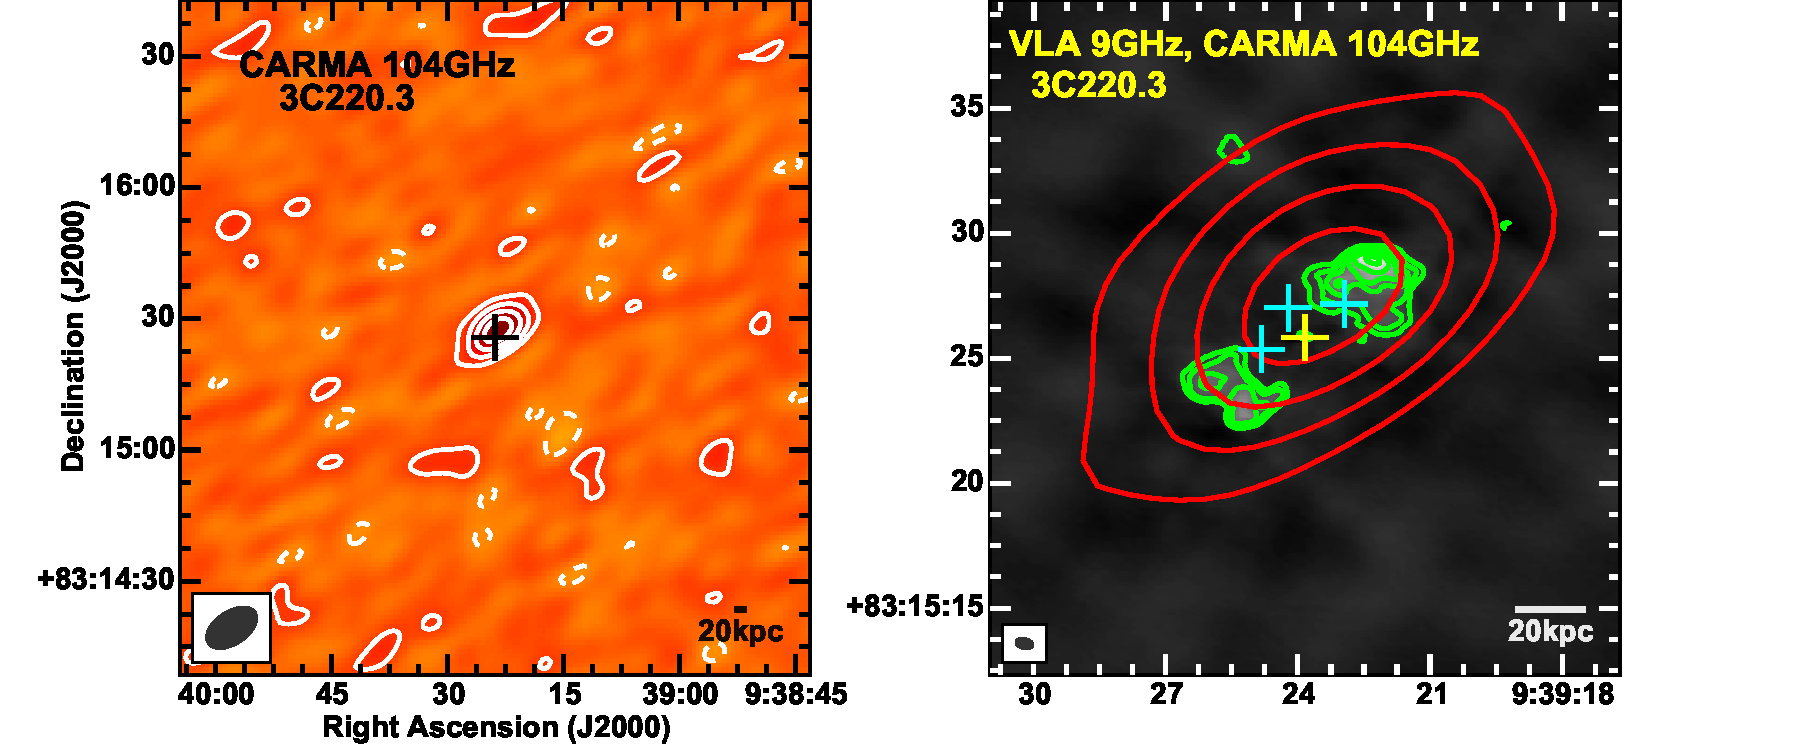
\includegraphics[width=0.80\textwidth]{Figure/ContPanel}
\caption{The central cross indicates the position of the radio core of 3C220.3. Contour levels of the 9 GHz continuum emission start at $\pm$4$\sigma$ of $\sigma$ = 0.0641 mJy beam$^{-1}$ and increment at steps of $\pm$2$^n\sigma$, where n is positive integers; contour levels of the 104 GHz continuum emission start at $\pm$3$\sigma$, incrementing at steps of $\pm$1$\sigma$ of 0.5 mJy beam$^{-1}$.
Left:Contour map of the 104 GHz continuum emission in 3C220.3. The beam size is 16\farcs67 $\times$ 7\farcs17, at P.A. = -58$\degr$, as indicated in the bottom left corner. Right: Contours of the CARMA 104 GHz continuum emission (red) from the foreground radio galaxy 3C220.3 overlaid the 9 GHz emission (green) \citep{Haas14}. The rms in the 9GHz image is $\sigma$ = 0.0641 mJy beam$^{-1}$. The synthesized beam size of the VLA observations is 0$\farcs$60 $\times$ 0$\farcs$23 at P.A. 76$\degr$. 
\label{fig:cont}}
\end{figure*}


\subsection{New results: CO($J$ = 3 $\rightarrow$ 2) line emission}
%peak 19.907623291015625 2.2045940408007811
%We have detected unresolved CO($J$ = 3 $\rightarrow$ 2) line emission toward SMM J0939+8315 at peak flux
%of blah sigma  of $ \sigma$ = blah mJy beam$^{-1}$.
We detect unresolved CO($J$ = 3 $\rightarrow$ 2) line emission toward the background SMG SMM J0939+8315. We extract the spectrum and fit a single-component Gaussian as shown in Figure \ref{fig:mom0}, yielding peak flux density of 19.90 $\pm$ 2.20 mJy, superimposed on a continuum level of 3.46 mJy, the FWHM of the Gaussian fit is 541.65 $\pm$ 31.91 km s$^{-1}$. The spatial extent of the SMG is shown in the SMA 1 mm dust continuum in Figure \ref{fig:mom0}, where the synthesized beam size of the SMA observation is 1\farcs42$\times$1\farcs16, at P.A. -34.0\degr. Since the angular resolution of our CO measurement is 13$\farcs$57 $\times$ 5\farcs77 , the CO($J$ = 3 $\rightarrow$ 2) detection in the SMG is therefore spatially unresolved. We construct the velocity-integrated (moment-0) map of the CO($J$ = 3 $\rightarrow$ 2) emission using the uv-continuum subtracted data, the velocity-integrated CO($J$ = 3 $\rightarrow$ 2) line flux is 14.6 $\pm$ 0.9 Jy km s$^{-1}$.

Channel width used for mom0 map. and to get the integrated flux.

\begin{figure*}[tbph] 
\centering
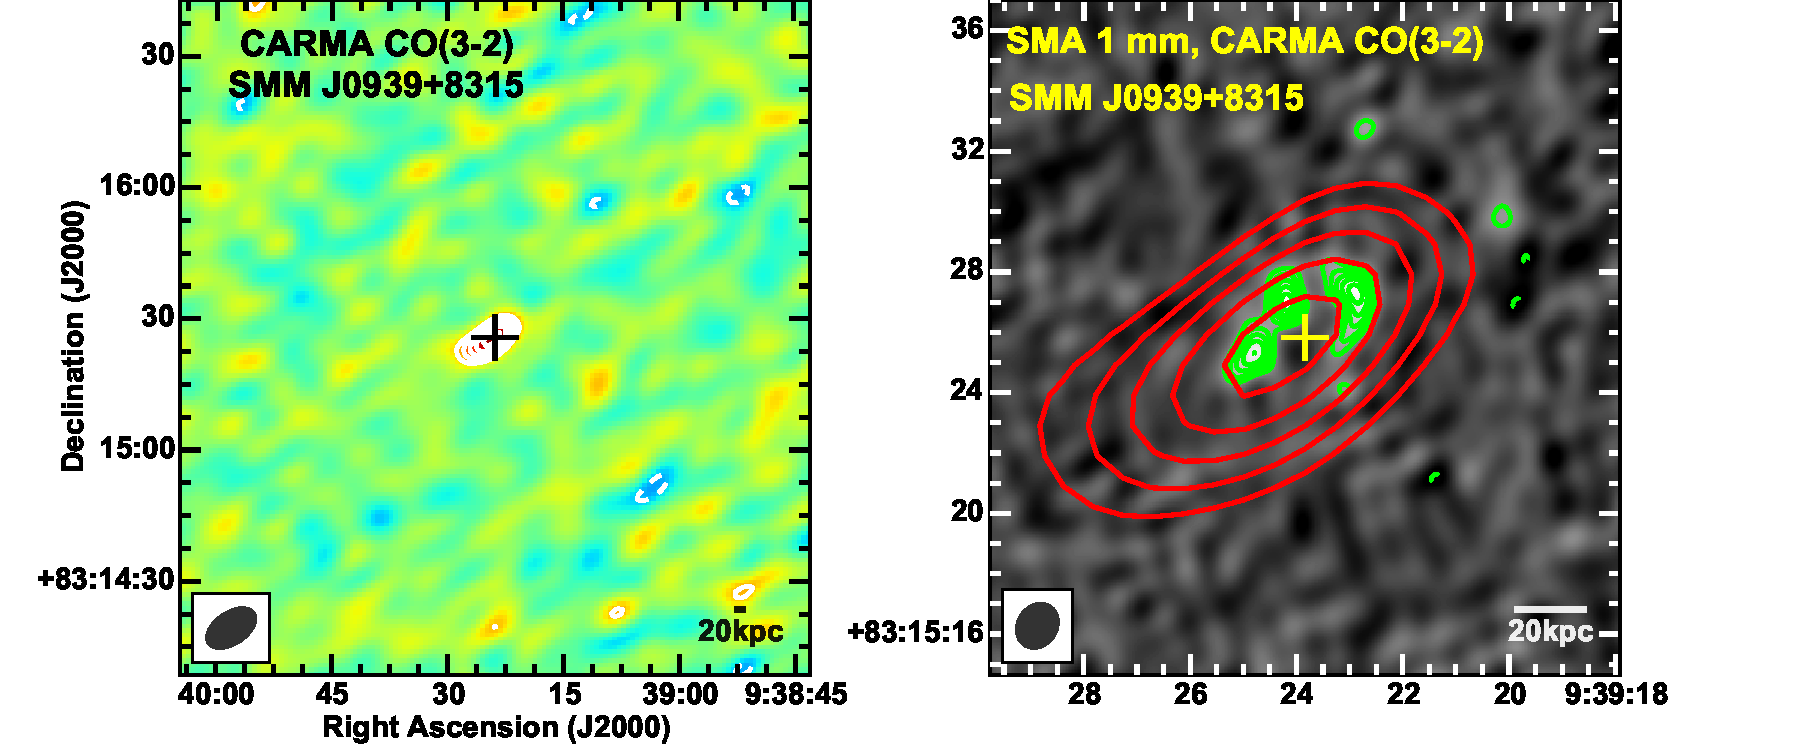
\includegraphics[width=0.8\textwidth]{Figure/LinePanel}
\includegraphics[width=0.65\textwidth]{Figure/peak28_WiderSpectrum}
\caption{The central cross represents the coordinates for alignment between plots. The contour starts at $\pm$3$\sigma$, incrementing at
steps of $\pm$1$\sigma$. Top Left: Continuum-subtracted moment-0 map of the CO($J$ = 3 $\rightarrow$ 2) line emission in the background SMG with $\sigma$ = 0.7 Jy km s$^{-1}$ beam$^{-1}$. The angular resolution is 13$\farcs$57 $\times$ 5\farcs77, the beam size is shown in the bottom left corner. 
Top Right: Contours of CO($J$ = 3 $\rightarrow$ 2) emission (red) overlaid on the SMA 1 mm dust continuum (green) with $\sigma$ = 0.84 mJy beam$^{-1}$. The beam size of the SMA data is 1\farcs42$ \times $1\farcs16, P.A. -34\degr, as shown in the bottom left corner. From this image, it is apparent that the extent of the background SMG is smaller than the beam size of the CARMA observations, hence the CO($J$ = 3 $\rightarrow$ 2) line detection is spatially unresolved.
%Bottom: The Gaussian-fitted line peak of CO($J$ = 3 $\rightarrow$ 2) is 23.36 $\pm$ 2.21 mJy (before continuum
%subtraction), and the integrated line flux over linewidth of $\sim$1000 km/s is 14.6 $\pm$ 0.9 Jy km s$^{-1}$
%(after continuum subtraction).  
Bottom: Solid black line shows our Gaussian fit to the CO ($J$ = 3 $\rightarrow$ 2) line profile. Yellow histogram shows the flux density as a function of velocity offset, where 0 km/s corresponds to $z$ = 2.2214. 
\label{fig:mom0}}
\end{figure*}


\section{Analysis}
\subsection{Lens Modelling} \label{sec:Lens} %ok except table and errors
To study the intrinsic properties of the background galaxy, we determine the magnification factor by performing
lens modeling using the SMA 1 mm archival data of this system. The lens modeling is carried out in the visibility
(uv-) plane using the updated version\footnote{commit: 7aee6276} of the publicly available software {\sc uvmcmcfit}
(Bussmann et al., 2015). The code uses affine-invariant Markov chain Monte Carlo (MCMC) to sample the posterior
probability density function (PDF) of the model parameters. In our lens model, the surface mass densities of both
lenses are represented by singular isothermal ellipsoid (SIE) profiles, and the source is assumed to have an
elliptical Gaussian profile. The code does not include an external shear parameter. \newline
We fix the phase center to coordinates ($\alpha$, $\delta$) (J2000) = (144.84809\degr, 83.25725\degr), the
offset positions of the lenses and source are referenced to this phase center. The primary lens (3C220.3) is
described by 5 free parameters: the angular offset relative to
the chosen phase center in the image ($\Delta \alpha_{\rm
lens0}$ and $\Delta \delta_{\rm lens0}$), the angular Einstein radius ($\theta_{\rm E,0}$), the
axial ratio ($q_{\rm lens0}$), and the position angle ($\phi_{\rm lens0}$). The secondary lens (companion B) is
described by 3 free parameters: $\theta_{\rm E,1}$, $q_{\rm lens1}$, and $\phi_{\rm lens1}$. The angular offset
of the secondary
lens is sampled with respect to ($\Delta \alpha_{\rm lens0}$ and $\Delta \delta_{\rm lens0}$) of
the primary lens.
The source (SMM J0939+8315) is parameterized by
6 free parameters: the position of the source relative to the
primary lens ($\Delta \alpha_{\rm s}$ and $\Delta
\delta_{\rm s}$), the total intrinsic flux density ($S$), the
effective radius ($r_{\rm s} = \sqrt{a_{\rm s} b_{\rm s}}$), the axial
ratio ($q_{\rm s}$ =  $b_{\rm s}/a_{\rm s}$), and the position angle
($\phi_{\rm s}$).
The total number of free parameters is $N_{\rm free}$ = 14. The best-fit model is obtained by maximizing the
Gaussian likelihood function $ \mathcal{L} $ according to:
\begin{equation}
    \mathcal{L} = \sum_{u, v}\left( \frac{|V_{\rm data} - V_{\rm
    model}|^2}{\sigma^2} + {\rm log}(2 \pi \sigma^2) \right)
\end{equation}
\noindent where $\sigma$ is determined from the scatter in the visibilities within a
single spectral window (natural weighting).

We initialize the positions and the Einstein radii of both lenses, and the position of the source using the
values of the best-fit lens model \citet{Haas14} performed on Keck K-band near-infrared image. For each of
these parameters, we impose a uniform prior in the range $\in\pm$3$\sigma$, where $\sigma$ is the uncertainty
reported in their paper. The axial ratios of the lenses are restricted to $q_{\rm lens} > 0.3$. We initialize 512
walkers and 6000 steps to identify the best-fit model parameters.
\begin{figure}[!tbpH]
\centering
\includegraphics[width=0.232\textwidth]{Figure/LensedSBmap_model_bestfit}
\includegraphics[width=0.232\textwidth]{Figure/LensedSBmap_residual_bestfit}
\caption{We perform lens modeling using the latest version of {\sc uvmcmcfit} on the SMA 1 mm continuum data.
In this two lenses model, we initialize the lenses' positions using the values reported by \citet{Haas14}. Left:
Grayscale: Our best-fit model assuming an elliptical Gaussian profile for the background SMG. Magenta ellipses:
Half-light area of the background SMG. Orange Lines: Critical curves of foreground lenses. Black dots: Positions of
the two lenses. Red contours: Observed SMA 1 mm continuum. The contours start at 2$\sigma$, incrementing at
steps of $\pm$2$\sqrt{\rm 2}\sigma$. Right: Solid contours show the positive residuals at the same levels and dashed contours
show the negative residuals. \label{fig:lens}}
\end{figure}

The resulting best-fit model as shown in Figure \ref{fig:lens} shows no significant bowls in the residual
image, and the knots (lensed emission) in the observed SMA data are well-reassembled with the best-fit model.
The best-fit model yields a magnification
factor of $\mu_{\rm 1mm}$ = 9.73 $\pm$ 1.38, this is consistent the reported value in Haas et al.
2014 within errors. The Einstein radii associated with the best-fit model for the two lenses are $\theta_{E}$ =
1.22 $\pm$ 0.01 (8.75 kpc at $z$ = 0.685) and $\theta_{E}$ = 0.73 $\pm$ 0.02 (5.23 kpc at $z$ = 0.685),
the corresponding masses within the Einstein radii are $M(\theta < \theta_{\rm E})$ = (4.90 $\pm$ 0.58) $\times$ 10$^{11}$ $M_{\odot}$ and $M(\theta < \theta_{\rm E})$ = (1.76 $\pm$ 0.33) $\times$ 10$^{11}$ $M_{\odot}$, respectively. All best-fit
parameters are listed in Table \ref{tab:lensParam}.
\begin{deluxetable}{l l r}[tbpH]
\tabletypesize{\scriptsize}
\tablecolumns{3}
\tablewidth{0pc}
\tablecaption{Lens modeling results}
\tablehead{
\multicolumn{2}{c}{Parameters} &
\colhead{Best-Fit Values}
\\ \cline{1-3} \vspace{-0.05in} \\
% \tableline
\multicolumn{3}{c}{Lens 0}
}
\startdata
%\cutinhead{Lens 0}
$\Delta \alpha_{\rm lens0}$      & (\arcsec)   & 0.403 $\pm$ 0.026     \\
$\Delta \delta_{\rm lens0}$      & (\arcsec)   & -0.181 $\pm$ 0.027    \\
$q_{\rm lens0}$ \tablenotemark{a} &             & 0.446 $\pm$ 0.063     \\
$\phi_{\rm lens0}$                & (deg)       & 31.56 $\pm$ 4.15\phn  \\
$\theta_{\rm E0}$                & (\arcsec)   & 1.218 $\pm$ 0.010     \\
\cutinhead{Lens 1}
$\Delta \alpha_{\rm lens1}$       & (\arcsec)   & -0.804 $\pm$ 0.034    \\
$\Delta \delta_{\rm lens1}$       & (\arcsec)   & -1.243 $\pm$ 0.017    \\
$q_{\rm lens1}$ \tablenotemark{a} &             & 0.608 $\pm$ 0.138     \\
$\phi_{\rm lens1}$                & (deg)       & 14.2 $\pm$ 15.7\phn      \\
$\theta_{\rm E1}$                & (\arcsec)   & 0.745 $\pm$ 0.015     \\
\cutinhead{Source}
$\Delta \alpha_{\rm s}$           & (\arcsec)   &  -0.163 $\pm$  0.035   \\
$\Delta \delta_{\rm s}$           & (\arcsec)   & -0.193 $\pm$  0.048   \\
$q_{\rm s}$ \tablenotemark{a}     &             & 0.424 $\pm$ 0.237     \\
$\phi_{\rm s}$                    & (deg)       & 174.34 $\pm$ 8.89\phn \\
$r$\tablenotemark{b}              & ($\arcsec$) & 0.106 $\pm$   0.033   \\
$\mu$                             &             & 10.13 $\pm$ 1.38\phn
\enddata
% 0.377 & -0.209 & 0.446 & 33.22 & 1.223 & -0.788 & -1.26 & 0.5289 & 9.55 & 0.733 & 9.74
\label{tab:lensParam}
\tablenotetext{a}{Axial ratio}
\tablenotetext{b}{Effective Radius}
% \tablenotetext{c}{}
\tablecomments{The angular offsets listed above are with respect to $\alpha$ = 9:39:23.54, $\delta$ = 83:15:26.10 (J2000). }
\end{deluxetable}

















\subsection{SED fitting} \label{sec:SED}
%Lensing system, both foreground and background objects contribute to the emission, especially at frequency near
%100 GHz.
\subsubsection{3C220.3}

We detect the radio continuum with peak flux density of S$_\nu$ = 5.56 $\pm$ 0.54 mJy at $\nu_{cont}$ = 104.2106 GHz (2.877 mm) in the observed-frame. In this lens system, the foreground galaxy (3C220.3) is a double-lobed FR-II radio galaxy, hence we expect the continuum to be dominated by synchrotron emission from the foreground galaxy. At this frequency, we expect the emission from the radio core to dominate our continuum detection; however, the integrated flux density is measured to be 7.18 $\pm$ 0.69 mJy. Considering the fact that the orientation of the synthesized beam aligns with the axis along the lobes of the foreground radio galaxy as shown in Figure \ref{fig:cont}, we interpret this difference between the peak flux density and the integrated flux density as the source (core and lobes) being partially resolved, i.e., the continuum detection includes non-thermal emission from the lobes. Besides, the contours of the 104 GHz continuum are
centered on the north lobe of the radio galaxy, this further supports our argument.
%% OK up


Talk about the radio core:
\citet{Mullin06a} report null detection of the radio core with upper limit of blah mJy at 4.6 GHz, whereas \citet{Haas14} report a detection of the radio core of 0.8 mJy at 9 GHz. 
We fit a functional form for the radio lobe to NED data following Equation (1) by \citet{Cleary07a}, extrapolate to continuum frequency = blah mJy. which is consistent with our continuum measurement. BLLAHHHH

We estimated the radio core contribution at our continuum frequency by taking two FR-II galaxies from the
3C catalog that have measurements on the radio core. 

%By calculating their core spectral index, we extrapolated the radio core emission of 3C220.3 to our continuum frequency to be blah mJy, implying the continuum is dominated by the radio lobe. 

Therefore the X $\sigma$ detection of the partially resolved continuum emission from the foreground radio galaxy suggests a 
non-negligible contribution coming from the lobe emission, the peak flux density therefore does not corresponds to the core emission.

\begin{figure}[!tbph]
\centering
\includegraphics[width=0.5\textwidth]{Figure/3C220_3FullSED}
\caption{Figure shows the SED of 3C220.3 and SMM J0939+8315 including the new measurements presented in this paper. 
Black markers represent existing data of 3C220.3 (see table \ref{tab:SEDdataRadio}). Red markers at 104 GHz corresponds to our continuum measurements (integrated, peak, and difference). The dashed black line corresponds to the parabolic function we fit to the data associated with the radio galaxy following \citet{Cleary07a} and references therein. The dashed blue line and the dashed dot magenta line correspond to the best-fit SED of the background galaxy using an optically thick model, and an optically thin model, respectively. \label{fig:SED}}
\end{figure}

\subsubsection{SMM J0939+8315} 
data listed in Table \ref{tab:SEDdataRadio}
\begin{deluxetable}{ccc}[tbpH]
\tabletypesize{\scriptsize}
\tablecolumns{3}
\tablecaption{SMM J0939 Photometry}
\tablehead{
\colhead{Wavelength ($\micron$)} &
\colhead{Flux Density (mJy)} &
\colhead{Instrument}
%\\ \tableline
%\multicolumn{3}{c}{SMM J0939 Photometry}
}
\startdata
70 & 29.5 $\pm$ 5 & PACS \\
100 & 102.0 $\pm$ 7 & PACS\\
160 & 289.0 $\pm$ 9 & SPIRE\\
250 & 440.0 $\pm$ 15 & SPIRE\\
350 & 403.0 $\pm$ 20 & SPIRE\\
500 & 268.0 $\pm$ 30 & SPIRE\\
1000 & 51.0 $\pm$ 12 & SMA
\enddata
\label{tab:SEDdataRadio}
%\tablenotetext{a}{}
\tablecomments{SED photometry from \citet{Haas14}}
\end{deluxetable}



%burn-in phase 100, walkers 500, steps 500,
To constrain the dust and gas properties in the ISM of SMM J0939+8315, we perform SED fitting based on the
photometric data obtained using the Spitzer Space Telescope and the {\it Herschel} Space Telescope, at wavelengths
between observed-frame 70 \micron-1000 \micron, and the SMA interferometric data at 1 mm. We use the publicly
available software {\sc mbb\_emcee} to perform SED fitting, the code uses an affine-invariant Markov chain Monte
Carlo (MCMC) approach, the details are described by \citet{Riechers13a, Dowell14a}. The
functional form comprises of a modified blackbody function with a power law S$_{\lambda} \propto \lambda^\alpha
$ attached to the blue
side.
We fit both an optically thick and optically thin model. In the optically thick case, the wavelength $
\lambda_0$ = $\frac{c}{\nu_0}$ is an additional parameter which represents where the optical
depth $\tau_{\nu}$ = ($\nu$/$\nu_0$)$^\beta$ reaches unity. Thus, the functional form of the modified blackbody
in the optically thick regime is as follows:
\begin{equation}
\rm S_{\lambda} \propto \frac{(1-exp^{-(\frac{\lambda_0 (1+z)}{\lambda})^{\beta}})(\frac{c}{\lambda})^3}
{exp^{\frac{hc}{\lambda\rm{kT/(1+z)} } }-1}
\end{equation}
and in the optically thin regime, the functional form reduces to:
\begin{equation}
\rm S_{\lambda} \propto \frac{(\frac{c}{\lambda})^{\beta+3}}{exp^{\frac{hc}{\lambda\rm{kT/(1+z)}}}-1}
\end{equation}
where T is the rest-frame characteristic cold dust temperature (fitting to the FIR part), $\lambda_0$ is rest-frame wavelength
where the optical depth reaches unity, $\beta$ is the dust emissivity (or spectral index of the dust extinction
curve), and $\alpha$ is the power law spectral index. The overall fit is normalized using the observed-frame 500
$\micron$ flux density, hence this becomes an additional parameter in the fit. In both models, we impose an upper limit on $\lambda_0$ to 2000 \micron, and the observed-frame dust temperature $T_{\rm d}/(1+z)$ to 60 K. We fix the upper limit on $\beta$ to be 3.0 and 2.2 for the optically thin model and optically thick model, respectively.
%; although this has minimal effects on the overall fit when we remove the upper limit, the best-fit $\beta$ does not dependent on this upper limit. << seems like it actually depend on the upper limit..
\begin{deluxetable}{ccc}[tbpH]
\tabletypesize{\scriptsize}
\tablecolumns{3}
\tablecaption{SED fitting results}
\tablehead{
\colhead{Parameters}                  &
\colhead{Optically Thick}       &
\colhead{Optically Thin}
}
\startdata
$\chi^2$ & 2.25 & 5.31 \\
D.O.F & 2 & 3 \\
$T_{\rm d}$ (K) & 60.91$^{+1.08}_{-1.31}$ & 51.95$^{+1.26}_{-1.21}$ \\
$\beta$ & 1.35$^{+0.57}_{-0.53}$ & 0.7$^{+0.24}_{-0.26}$ \\
$\alpha$ & 3.05$^{+0.31}_{-0.40}$ & 2.76$^{+0.23}_{-0.23}$ \\
%$\lambda_0$(1+$z$) ($\micron$) \tablenotemark{c} & 722.81$^{+276.88}_{-398.67}$ & --- \\
$\lambda_0$ ($\micron$) \tablenotemark{e} & 224.41$^{+85.96}_{-123.77}$ & --- \\
$\lambda_{\rm peak}$ \tablenotemark{c}\micron & 254.7$^{+6.2}_{-6.1}$ & 301.4$^{+29.0}_{-30.1}$ \\
$f_{\rm norm, 500 \micron}$ mJy  \tablenotemark{c} & 255.79$^{+16.67}_{-16.31}$ & 244.25$^{15.28}_{15.30}$ \\
$L_{\rm (8-1000)\micron}$ [10$^{12}$ L$_\sun$] \tablenotemark{d} & 88.52$^{+2.62}_{-2.63}$ & 89.15 \\
$M_{\rm d}$ [10$^8$ M$_\odot$] \tablenotemark{b} & 50.47$^{+20.42}_{-20.15}$ & 25.74$^{+3.88}_{-5.49}$
\enddata

% Optically thick & 18.91 & 1.35 & 722.81 & 3.05 & 254.7 & 88.52 & 50.47 \\
% Optically thin &  16.13 & 0.7 & N/A   & 2.76 & 301.4 & 89.15 & 25.74

\label{tab:mbb}
\tablenotetext{a}{The observed-frame wavelength where the dust becomes optically thick}
\tablenotetext{b}{Assuming standard absorption mass coefficient $\kappa$=2.64 m$^2$ kg$^{-1}$ at $\lambda$=125.0 $\micron$ (Dunne et al. 2003), without lensing correction}
\tablenotetext{c}{observed-frame}
\tablenotetext{d}{rest-frame 8-1000 $\micron$ without lensing correction}
\tablenotetext{e}{The rest-frame wavelength where the dust becomes optically thick, upper limit is 2000 $\micron$}
\tablecomments{Errors are $\pm$1$\sigma$}
\end{deluxetable}

% thick_500_500.log
% T/(1+z): 18.91 +1.09 -1.31 (low lim: 1.00 upper lim: 60.00) [K]
% beta: 1.35 +0.57 -0.53 (low lim: 0.10 upper lim: 2.20)
% fnorm: 255.79 +16.67 -16.31 (low lim: 0.03) [mJy]
% lambda0 (1+z): 722.81 +276.88 -398.67 (low lim: 1.00 upper lim: 3049.15) [um]
% alpha: 3.05 +0.31 -0.40 (low lim: 0.10 upper lim: 20.00)
% Lambda peak: 254.7 +6.2 -6.1 [um]
% L_IR(8.0 to 1000.0um): 88.52 +2.62 -2.63 [10^12 L_sun]
% M_d(kappa=2.64, lam=125.0um): 50.47 +20.42 -20.15 [10^8 M_sun]
% Number of data points: 7
% ChiSquare of best fit point: 2.25

% note using beta upper limit 3.0, getting very different beta, and dust mass
% Fit results:
% T/(1+z): 19.75 +0.56 -0.53 (low lim: 1.00 upper lim: 60.00) [K]
% beta: 1.91 +0.76 -0.76 (low lim: 0.10 upper lim: 3.00)
% fnorm: 267.13 +16.03 -15.98 (low lim: 0.03) [mJy]
% lambda0 (1+z): 1012.99 +142.79 -275.29 (low lim: 1.00 upper lim: 3049.15) [um]
% alpha: 3.64 +0.08 -0.86 (low lim: 0.10 upper lim: 20.00)
% Lambda peak: 255.6 +6.3 -6.2 [um]
% L_IR(8.0 to 1000.0um): 88.02 +2.85 -2.85 [10^12 L_sun]
% M_d(kappa=2.64, lam=125.0um): 108.23 +32.00 -63.67 [10^8 M_sun]
% Number of data points: 7
% ChiSquare of best fit point: 2.25
% Saving results to thick_testbeta.h5

% thin_testSMA
% T/(1+z): 16.13 +1.26 -1.21 (low lim: 1.00 upper lim: 60.00) [K]
% beta: 0.70 +0.24 -0.26 (low lim: 0.10 upper lim: 3.00)
% fnorm: 244.25 +15.28 -15.30 (low lim: 0.03) [mJy]
% alpha: 2.76 +0.23 -0.23 (low lim: 0.10 upper lim: 20.00)
% Lambda peak: 301.4 +29.0 -30.1 [um]
% L_IR(8.0 to 1000.0um): 89.15 +2.48 -2.51 [10^12 L_sun]
% M_d(kappa=2.64, lam=125.0um): 25.74 +3.88 -5.49 [10^8 M_sun]
% Number of data points: 7
% ChiSquare of best fit point: 5.31

The best-fit values in both regimes are listed in Table \ref{tab:mbb}. The best-fit solution of an optically thin
model corresponds to $\chi^2$ = 5.31 with 3 degrees of freedom, whereas that of an optically thick model
corresponds to $\chi^2$ = 2.25 with 2 degrees of freedom, suggesting a better fit than the optically thin
model. In the remaining analysis, we employ the inferred values from the optically thick model.
The best-fit solution yields a FIR luminosity of $L_{\rm FIR (42.5-122.5\micron)}$ = 53.33$^{+1.14}_{-1.13}\times$10$^{12}L_\odot$, and a total IR luminosity of $L_{\rm IR (8-1000 \micron)}$ = 88.52$^{+2.62}_{-2.63}\times$10$
^{12}L_{\odot}$. Assuming a dust absorption coefficient of $\kappa_{\nu}$ = 2.64 m$^2$ kg$^{-1}$ at 125.0 $
\micron$ (e.g., Dunne et al. 2003), we derive the dust mass using the following expression:
\begin{equation}
\mathrm{M_{\rm dust}} = S_{\nu} \times D_{L}^2 [(1 + z) \kappa_{\nu} B_{\nu}]^{-1} \times \tau_{\nu} [1-
\exp(-\tau_{\nu})]^{-1}
\end{equation}
where $S_{\nu}$ is the flux density, $D_{\rm L}$ is the luminosity distance, $\kappa_{\nu}$ is the dust
absorption coefficient, $\tau_{\nu}$ is the optical depth, and $B_{\nu}$ is the Planck function,
all quantities are expressed in the observed-frame. We find a dust mass of $M_{\rm dust}$ =
50.47$^{20.42}_{-20.15}\times$10$^8 M_{\odot}$. These values are based on photometric data, i.e. prior
to lensing correction.

NOTE:
using beta upper limit 3.0, getting very different beta, and dust mass dot dot dot

\begin{figure}[!tbp]
\centering
\includegraphics[width=0.5\textwidth]{Figure/CorrelationPlot__thick_testbeta}
\includegraphics[width=0.5\textwidth]{Figure/CorrelationPlot__thin_testSMA}
\caption{Resulting correlation plot from our SED fitting. Plots on the diagonal axes are marginalized posterior probability distribution of each
parameter. Off-diagonal plots are 2D histograms between parameters. Cross denotes where the best-fit value corresponds to in the 2D correlation plot. Top: Optically thick
model. Bottom: Optically thin model. The parameter T is the observed-frame characteristic dust temperature.\label{fig:sedlikelihood}}
\end{figure}
%Our uncertainties on M$_{d}$ do not include the uncertainty in $K_{\nu}$, which is at least a factor of blah dex.
%In most cases, $\alpha$ is poorly constrained, with the fits only providing a lower limit. Because of the way the
%blue-side power law is joined to the MBB,
%this simply amounts to a statement that the merge point between the power law and the thermal SED lies at
%wavelengths lower than the shortest
%wavelength photometry point (250 micron). (in Dowell et al. 2014)
% Compare to Haas SED
%The SED based on the dust emission of the background SMG in 250-1000 $\micron$ is best fitted with dust
%temperature T$_{\rm d}$ $\sim$ 36 K at z = 2.221 fixing dust emissivity index $\beta$ = 1.5,
%their the intrinsic FIR luminosity from the background source is L$_{\rm FIR}$ = 1 $\times$ 10$^{13}$ L$_{\odot}$


\subsection{Radio-FIR correlation}%%%%% ok, except add comparison.
% q correlation using IR: 2.81
We extrapolate the flux density at rest-frame 100 GHz based on the optically thick model; assuming a power law
spectral index of -0.8 in the radio domain of the SED, we calculate the corresponding rest-frame luminosity $L_{\rm 1.4}$. Together with the
integrated FIR luminosity with lensing correction, we derive the radio-IR correlation parameter (q) using:
\begin{equation}
q = \log{10} \frac{L_{\rm FIR}} {9.8\times10^{-15}} L_{\odot} - \log{10}\frac{L_{\rm 1.4}} {\rm W\ Hz^{-1}}
\end{equation}
This yields $q$ = 2.59 $\pm$ blah.
Compare to other galaxies blah. to be expanded -- hwhatjhoaenthajkegnakrgneargkea
%$S_{\rm 1.4 GHz}$ = 0.45655848 mJy / mu (observed frame) mJy

\subsection{Molecular gas mass}
%Equation: M$_gas$ = alpha$\times$L$_{\rm CO}$
Talk about the brightness temperature ratio $<$ 1 for SMG, and $\sim$ 1 for quasar, so we adopt 1 here since the source is hosting a quasar.

Frayer: Observations of CO(1-0) are key for deriving the total molecular gas mass. The CO(1-0) line traces the cold material not probed by the higher-level CO transitions. Unfortunately, most high-redshift sources to date have been observed in only the higher level J > 1 transitions, and many papers have assumed a single-component ISM that is fully thermalized with Tb (J>1) / Tb (1-0) = 1. However, recent CO(1-0) observations of the SMG population show that this assumption is not correct (e.g., Harris et al. 2010, Carilli et al. 2010; Swinbank et al. 2010; Ivison et al. 2010, and 2010). From the compilation of these previous results, an average CO line ratio value of R31 = 0.6 pm 0.1 is found for a sample of nine SMGs. 

Since only CO($J$ = 3 $\rightarrow$ 2) line has been detected on this object, we derive the molecular gas mass in
this SMG assuming thermalized excitation or assuming thermalized optically thick CO, i.e. the brightness temperature ratio between CO($J$ = 3 $\rightarrow$ 2)
and ($J$ = 1 $\rightarrow$ 0) is $R_{31}$ = 1 (e.g., Riechers et al. 2011; Ivison et al. 2008, 2012; Scott et
al. 2011). We calculate the CO($J$ = 1 $\rightarrow$ 0) line luminosity using standard relations (e.g., Solomon \&
van den Bout 2005; Carilli \& Walter 2013):
\begin{equation}
L^{\prime}_{\rm CO} = \frac{3.25\times10^7}{\nu_{\rm CO (3-2), rest}^2}\times \frac{D_L^2}{\mu} \times
\frac{I_{\rm CO(3-2)}} {R_{\rm 31} (1 + z)}
\end{equation}
this corresponds to $L^{\prime}_{\rm CO (1-0)}$ = (4.13 $\pm$ 0.87) $\times$ 10$^{10}$ ($\mu$/9.74)$^{-1}$ [\rm K km s$^{-1}$ pc$^2$]
after lensing correction. The inferred total molecular gas mass is therefore M$_{\rm gas}$ = 3.303$\times
$10$^{10}$ ($\alpha$/0.8) ($\mu$/9.74)$^{-1} M_\odot$. We assume a conversion factor of $\alpha_{\rm CO}$ =
0.8 M$_\odot$ (K Km s$^{-1}$ pc$^2$)$^{-1}$ based on empirical relations from local ULIRGs, which is typically
adopted for SMGs \citep{Bothwell13a,Tacconi10a,Daddi2010a}. As derived in the previous section, SMM has a dust mass of M$_{\rm dust}
$=50.47$^{20.42}_{-20.15}\times$10$^8\rm M_{\odot}$ (before lensing correction), this corresponds to a gas-to-dust
ratio of f$_{\rm gas-dust}$ = $M_{\rm gas}/M_{\rm dust}$ = 63.74 $\pm$ blah , which is in good agreement with the range of values found in other SMGs (cite).



Follow-up CO(1?0) observations of three representative z ? 1.5 galaxies in the CO(1?0) line emission suggest that the molecular gas in these systems is already sub-thermally excited at the CO(3?2) transition similar to what is found in local disks (Dannerbauer et al. 2009; Aravena et al. 2010), with typical line brightness temperature ratios between both lines of ? 0.5. This is also similar to what is found in SMGs (Harris et al. 2010; Ivison et al. 2011; Bothwell et al. 2013), but substantially different to high-redshift QSOs, which appear to have highly excited gas with line temperature ratios close to unity (Riechers et al. 2006; Wei� et al. 2007; Ao et al. 2008; Riechers et al. 2011a; Ivison et al. 2012, e.g.,). Recent observations of z ? 0.3 disk galaxies support these findings, indicating that the molecular gas content, as traced by CO(1?0), is two times larger than expected from J > 3 CO measurements, comparable to z > 2 SMGs (Papadopoulos \& Ivison 2002; Harris et al. 2010; Ivison et al. 2011; Riechers et al. 2011c). 
% Michalowski et al. 2010, Santini et al. 2010
% typical of local ULIRs is ~ 100)
%\citep{Riechers2011a}


\subsection{Star formation rate} %%% ok, except comparison
We derive the star formation rate (SFR) using the modified Kennicutt (1998) relation, assuming a Chabrier (2003)
stellar initial mass (IMF) function: SFR = 1.0 $\times$ 10$^{-10}\times$ ($L_{\rm IR\ or\ FIR}$). This yields SFR$_{\rm IR}$ = (909.12$\pm$155.67) $\times\ (\mu/9.74)^{-1}$ [$M\sun$ yr$^{-1}$] and SFR$_{\rm FIR}$ 547.71$\times(\mu/9.74)^{-1}$ [M$\sun$ yr$^{-1}$] using lensing-corrected (far-)infrared luminosities (L$_{\rm IR}$ and L$_{\rm FIR}$) derived from our SED fitting, and assuming negligible contribution from AGN.

Assuming constant SFR, the minimum time for which the starburst in SMM J0939+8315 can be maintained at its
current SFR is approximated by the gas depletion timescale $\tau$ = M$_{\rm gas}$/SFR, which is $\tau_{\rm IR}$ = 36.33 Myr, and $\tau_{\rm FIR}$ = 60.30 Myr.
Compare THIS NUMBER: with other SMGs (e.g., \citep{Greve05a}).


\subsection{SFE}
%SFE using LIR: 220.22
%SFE using LFIR: 132.68
% The ratio between LIR ($\propto$ SFR) and L$^\prime$CO ($\propto$ Mgas)
Frayer: Since the IR luminosity is proportional to the SFR and the CO L is proportional to the molecular gas mass, the IR-to-CO L ratio provides an indication of the SFE. Strong starburst and ULIRGs tend to show high IR-to-CO L ratios of $gtsim$ 100 L$\sun$ ( K km/s pc2)-1 (e.g., Solomon \& Vanden Bout 2005). Greve et al. (2005) found an average L(IR)/L$\prime$CO ratio for SMGs which was a factor of two larger than that for local ULIRGs



The SFR per unit mass of molecular gas is commonly taken as a
measure of the star formation efficiency, SFE = SFR/M$_{\rm gas}$. We compute the ratio using lensing-corrected (far-)infrared luminosities (L$_{\rm IR}$ and L$_{\rm FIR}$) and CO($J$ = 1 $\rightarrow$ 0) luminosity SFE = L$_{\rm F/IR}$/L$^\prime_{\rm CO(1-0)}$, this ratio makes no assumptions on the gas mass conversion factor $\alpha$ and is independent of the choice of IMF,
assuming no differential lensing between the CO and infrared emission.



or IR-to-CO line L ratio
Fix comparison HERE blah blah blah blah

We find a ratio of SFE$_{\rm IR}$ = 220.22 and SFE$_{\rm FIR}$ = 132.68, which are comparable
to what is found in "typical" SMGs (tacconi et al. 2006, Riechers et al. 2010, cite).
Note: SFE values for ULIRGs and distant SMGs typically exceed 100 L$_\odot$ [K km/s pc$^2$]$^{-1}$
(e.g., Yao et al. 2003; Neri et al. 2003; Greve et al. 2005; Bouche et al. 2007).



\subsection{Dynamical mass} %% check half light radius error, and comparison
We derive the dynamical mass of SMM J0939+8315 using an isotropic virial estimator (e.g., Engel et al. 2010):
\begin{equation}
M_{\rm dyn} = 2.8\times 10^5 \times \Delta \rm v_{\rm line}^ 2 \times r\ [kpc]
\end{equation}
where the line width $\Delta \rm v_{\rm line}^ 2$ is based on our CO($J$ = 3 $\rightarrow$ 2) line
measurement and the half-light radius is based on our lens model, $r$=0\farcs023484 $\pm$ 0\farcs033. This yields gas-to-dynamical mass fraction of f$_{\rm gas-to-dyn}$ = 2.03.


Compare to other. blah blah blah dynamical mass?, is it consistent with molecular gas mass?

\subsection{Surface mass density}

\section{Discussion} \label{sec:conclusions}
We present blah...

A lensed SMG that is likely to be hosting a type-2 quasar, this source offers an exceptional opportunity to
investigate the gas mass and dynamics of this
poorly-studied population of high z galaxies.


In this paper, we present blah of a strongly lensed blah at z = 2.221, at the epoch of cosmic star formation (cite)
This paper focuses on a blah source J0939+8315, a lensing galaxy.
We report a detection of CO($J$ = 3 $\rightarrow$ 2) line  blah $\sigma$ of $\sigma$ = blah (mJy) / beam (over a channel width of blah km/s); and continuum of blah $\sigma$ of $\sigma_{cont}$ = blah [mJy / beam].
The continuum detection is marginally resolved, we place constraints on the SED of the foreground galaxy (accounting for radio core and lobes emission).


We perform lens modelling to get magnification factor of blah.

We perform SED fitting of the SMG to get M$_{\rm dust}$, L$_{\rm FIR}$ of blah, L$_{\rm IR}$ of blah, yielding SFR of blah . Comparing our findings to other SMGs / similar populations, we find blah, which is blah.

look at "Lensed QSOs at high z observational, CO measurements (DB)" note

%\acknowledgments
%Facilities: \facility{CARMA}

\bibliographystyle{apj}
\bibliography{J0939}

%%% Will be replaced with table_compareSMG.tex


\begin{deluxetable*}{cccccccccc}[!tbp]
\tabletypesize{\scriptsize}
\tablecolumns{10}
\tablecaption{Properties of star-forming type-2 QSO host SMG -- SMM J0939+8315}
\tablehead{
\colhead{L$_{\rm IR}$} &
\colhead{L$_{\rm FIR}$} &
\colhead{SFR$_{\rm FIR}$} &
\colhead{q$_{\rm FIR}$\tablenotemark{d}} &
\colhead{SFE} &
\colhead{M$_{\rm gas}$\tablenotemark{c}} &
%\colhead{I$_{\rm CO (3-2)}$} &
%\colhead{I$_{\rm CO (1-0)}$} &
\colhead{L$^\prime_{\rm CO(1-0)}$\tablenotemark{b}} &
\colhead{$\tau_{\rm depl}$} &
\colhead{f$_{\rm gas-dust}$} &
\colhead{$f_{\rm gas-dyn}$\tablenotemark{a}}
\\
\colhead{(10$^{12}$ L$_\odot$)} &
\colhead{(10$^{12}$ L$_\odot$)} &
\colhead{(M$_\odot$ yr$^{-1}$)} &
\colhead{}  &
\colhead{(Myr$^{-1}$)} &
\colhead{(10$^{10}$M$_\odot$)} &
%\colhead{(Jy km s$^{-1}$)} &
%\colhead{(Jy km s$^{-1}$)} &
\colhead{(10$^{12}$ K km s$^{-1}$ pc$^2$)} &
\colhead{(Myr)} &
\colhead{}  &
\colhead{}
}
\startdata
88.52 & % before lensing correction
53.33 & % ditto
547.71 &
2.59 &
132.68 &
3.303 & % after correction
%14.60 &
%1.6222 &
4.13 & % after correction
60.30 &
63.74 & % after correction
2.03
\enddata
\label{tab:SMMprop}
\tablenotetext{a}{assuming half light radius of lens model of dust continuum}
\tablenotetext{b}{R$_{31}$ = 1}
\tablenotetext{c}{$\alpha_{\rm co}$ conversion 0.8}
\tablenotetext{d}{$\alpha_{\rm radio}$ spectral for -0.8}
\tablecomments{add errors; using optically thick model }
\end{deluxetable*}



\end{document}

